\section{Introduction}
\label{sec:cvpr_intro}

\dropcap{E}{vent} cameras capture per-pixel brightness changes at microsecond resolution, while consuming only milliwatts of power~\cite{gallego2020eventbased}. This combination enables low-latency perception and decision-making on agile but resource-constrained platforms such as small drones.

\begin{figure}[!t]
	\centering
	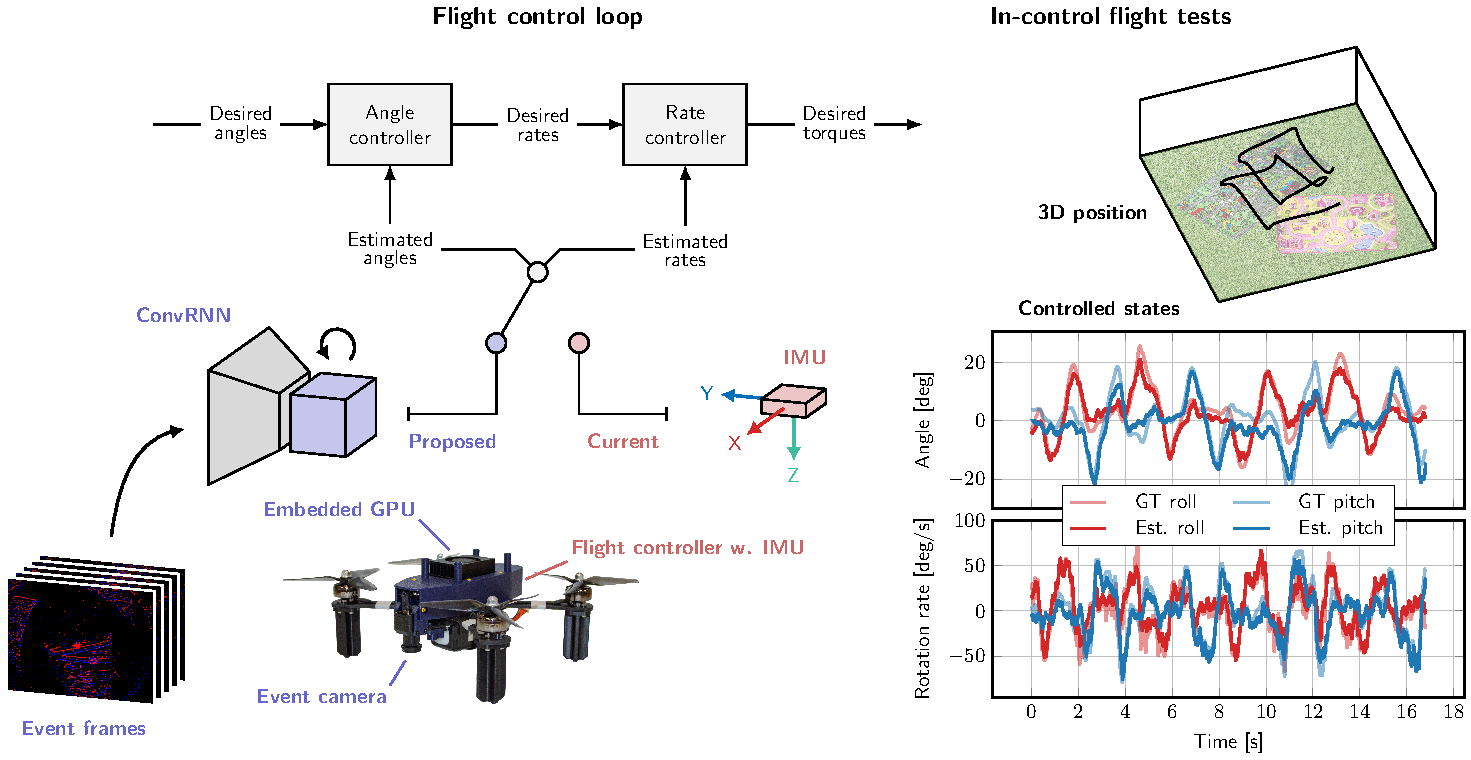
\includegraphics[width=\linewidth]{04_chapters/CVPR25/cc_figures/tikz-figure0.pdf}
	\caption{Online, on-device learning allows robots to ``train in their test environment''. We improve the time and memory efficiency of the self-supervised contrast maximization pipeline, such that on-board learning of monocular depth from event camera data becomes possible. When deployed on a small drone, online learning leads to better depth estimates and more successful obstacle avoidance behavior.}
	\label{fig:cvpr_overview}
\end{figure}

To make full use of the temporal information in the event stream, the learning pipeline consisting of network architecture and loss function should also operate at high frequency~\cite{paredes-valles2023taming}. Ground truth optical flow or depth is often only available at lower rates of 10-20~Hz~\cite{zhu2018multivehicle,gehrig2021dsec,chaney2023m3ed}. While some datasets allow upsampling of ground truth to higher rates~\cite{zhu2018multivehicle,burner2022evimo2}, reaching the temporal resolution of an event camera might be difficult and come at the cost of high data rates. This holds back supervised learning at the short time scales perceivable with event cameras. 

Contrast maximization~\cite{gallego2018unifying} allows self-supervised learning (SSL) of optical flow, depth and ego-motion from events alone~\cite{zhu2019unsupervised,paredes-valles2023taming,shiba2024secrets,gallego2019focus}. Since no ground truth is needed, learning and prediction can run at higher frequencies of 100~Hz~\cite{paredes-valles2023taming} or even 200~Hz~\cite{paredes-valles2024fully}, with the main limiting factor being the network's ability to integrate information over increasingly sparse inputs as the rate increases.

A major advantage of SSL is that it foregoes the costly process of obtaining ground truth, which enables learning to scale to large unlabeled datasets. An additional, but typically less emphasized advantage is that SSL can in principle be performed in the operational environment of a robot or other edge device. Such \emph{online} SSL greatly reduces the need for generalization of the learned model, as training happens directly on data sampled from the test distribution~\cite{vanhecke2018persistent}. For visual tasks like monocular depth estimation, this is particularly important, as generalization of this perceptual capability to environments different from the training environment is notoriously difficult~\cite{vodisch2023codeps,fu2024dectrain}.

Online SSL, however, introduces additional challenges. Chief among them is that not only the network but also the learning framework should be computationally efficient enough to run on board. In this chapter, we improve the efficiency of the contrast maximization pipeline such that on-device learning of low-latency monocular depth and ego-motion becomes feasible. This approach is visualized in \cref{fig:cvpr_overview}. We demonstrate continual learning of this complex visual task on board a small flying drone, and show the usability of the resulting depth for obstacle avoidance. Furthermore, we investigate various combinations of pre-training and on-board learning. When trained on event camera datasets, our small recurrent network shows state-of-the-art depth estimation performance among self-supervised approaches. Our work taps into the unused potential of on-board, online SSL, promising smaller reality gaps, leading to better performance.
